\chapter{Code Generation and Runtime Code}

\label{chapt:coderuntime}

\section{Using Kleene \fsm{}s in Real Projects}

 
You can build \fsm{}s using Kleene scripts and interactive \acro{gui} sessions,
and you can
use various commands, notably \texttt{test}, to 
test your \fsm{}s manually inside the Kleene \acro{gui}.


\begin{Verbatim}
test $MyFsm ;
\end{Verbatim}

\noindent
You have learned that these \fsm{}s can also be stored to file in \init{dot} and \xml{}
formats; and the \xml{} files can even be read back into Kleene, or shared with other
Kleene programmers.  However, an \init{xml} representation of
an \fsm{} is not executable code---it doesn't actually do anything by itself.  Even an
\fsm{} residing in memory is just a data structure consisting of nodes and arcs, and again it
doesn't do anything at all by itself.  An \fsm{} needs to be \emph{applied} to input, and
the output needs to be retrieved, by code that is derived from or exterior to the \fsm{} itself.

In order for your \fsm{}s to
be incorporated and used in projects external to the Kleene development environment itself,
we need to do one or both of the following:

\begin{itemize}
\item
Write \emph{runtime code} that reads in a Kleene \fsm{}, e.g.\@
from an \init{xml} representation, 
rebuilds the \fsm{} in memory, applies it to input and retrieves the output.
Such runtime code, probably implemented in a library in Java, \CPP{}, Python or whatever, could be
imported and used by application programs.
\item
Or, write scripts that take a Kleene \fsm{} and convert it into stand-alone
executable code that has the same behavior as the runtime code.
\end{itemize}

At this time, there is no runtime code available to load and run the \fsm{}s created
in Kleene.  Perhaps an interested developer would volunteer to write such code.  However, I (Ken
Beesley) have written some experimental \init{xslt} scripts that take a ``state-oriented''
\init{xml} file saved by Kleene and convert it into executable Java code (a Java package)
that can be imported
and used inside a larger program.  It is thus easy to incorporate your \fsm{}, e.g.\@ a
transducer that performs morphological analysis, inside any program written in the Java language,
or in any program written in Scala, Groovy or Clojure, which are also based on the Java Virtual Machine
(\init{jvm}) and so can use Java classes.

In the future, it should be possible to convert Kleene \fsm{}s into classes in other languages,
e.g.\@ \CPP{} and Python.

I will first discuss the current status and usage of the ``fst2java'' project, which generates
executable code in Java, and then give a high-level view of the requirements for runtime code.

\section{The fst2java Experiment}

\subsection{Stand-Alone Java Code Generation}

There is an experimental project called \emph{fst2java} that takes
a Kleene \fsm{}, stored to file in a \emph{state-oriented \init{xml} format}, and runs
this \init{xml} file through a set of \init{xslt} scripts, ultimately generating a Java package
that implements the \fsm{} as executable Java code.  This generated code performs \emph{complete
matching} of an input string, suitable for applications including tokenization and morphological
analysis, and returns a set of result strings for each successfully (completely) matched input
string.

The current fst2java project does not implement partial matching,
which would be suitable for applications such as entity extraction inside large input strings.

Once an \fsm{} has been stored to file, e.g. as \texttt{MyFst.xml}, and converted to 
a Java package, e.g.\@ \texttt{MyFstPackage}, containing a class definition
\texttt{MyFst.java}, then any Java (or Scala, Groovy or Clojure) program can simply

\begin{itemize}
\item
Import the \texttt{MyFst} package/class
\item
Create an instance of the class, and
\item
Call methods of the class to pass in input strings and various options, and get back the
results
\end{itemize}

\noindent The strings passed as input to the class methods are normal Java String objects, and the
methods inside the class are generated to convert these String objects automatically into lists of
code point values, taking into consideration any multi-character symbols in the alphabet of the
original \fsm{}.  A variety of public class methods are defined to accept String input and return
the results either as set (Java \texttt{ArrayList}) of Strings or as a marked-up \init{xml} string.

\subsection{How it Works}

\subsubsection{States Translate to Functions}

Recall that a Kleene \fsm{} consists of a finite number of states, one of which is designated as
the start state, and zero or more of which are final states; and each state has zero or more exit
arcs, each with an upper label and a lower label and a weight, leading to a destination state.  In a
high-altitude overview, fst2java translates each state in the \fsm{} into a Java function that
looks at the next input symbol in the input and tries to match that symbol to an upper or
\emph{input} label (``input'' in the OpenFst visualization of \fsm{}s) on one or more exit arcs.
For each matching exit arc, it calls the function representing the arc's destination state, passing
the remainder of the input string.  Functions representing final states also check, when first
called, to see if the input is exhausted, and if so, record a successful full match.

The scheme is complicated by weights, arcs with epsilon labels, which have to be ``explored''
without consuming any input, and by arcs labeled with \acro{other} symbols, which match
any input symbol that is not in the alphabet of the \fsm{}.  These complications are all
taken care of in the generated code, and the Kleene/Java programmer only needs to learn
the \init{api}, that is, the set of public methods available in the
generated class.

\subsubsection{Generation}

The fact that the generated Java code matches input symbols against \emph{upper}-side labels
(``input'' labels in the OpenFst visualization), means that the \fsm{} is effectively being applied
in a \emph{downward} direction, what the Xerox visualization of \fsm{}s calls \emph{generation}
mode.  However, if you have built a typical Xerox-style \fst{} morphological analyzer, i.e.\@
an \fst{} that has analysis strings (consisting of citation forms and tag symbols) on the upper side,
and orthographical strings on the lower side, and you want to generate Java code that accepts
orthographical strings and returns analysis strings, then all you need to do is to \emph{invert}
the \fst{} before generating the state-oriented \init{xml} file.  Then the input side (in the
OpenFst visualization) will contain orthographical strings, the string input will be matched on
that input side, the output side will contain the analysis strings (consisting of baseforms
and tags), and the Java code will work as expected.

Again, it is vitally important to understand that a Java class generated by fst2java from a Kleene
\fsm{} operates only in the downward or
generation direction as just described.  The input will be matched on the \emph{upper} side, what
the OpenFst tradition calls the \emph{input} side. 

If, in your Java code, you want to apply an
original \fst{} in both the downward (generation) and upward (analysis) directions, then
you need to generate two separate Java classes:

\begin{enumerate}
\item
One from the original \fst{}, perhaps resulting in \texttt{MyFstPackage/MyFst.java}, and
\item
Another from the inverted \fst{}, perhaps resulting in
\texttt{MyFstInvertedPackage/MyFstInverted.java}
\end{enumerate}

\noindent
Then your Java code could import both the \texttt{MyFst} and \texttt{MyFstInverted} packages/classes, calling one to
correspond to generation with the original \fst{}, and the other to correspond to analysis
with the original \fst{}.

\subsection{How to Create the Java Class Files for an \fsm{}}

\subsubsection{Status}

The fst2java project is still experimental and is not well tested.  It is not yet wired
into the Kleene \acro{gui}, and it will not be until it stabilizes and is better tested.  For now,
users who want to generate Java classes will need to follow the steps listed below, which hopefully
aren't too onerous.  The generation of Java code is performed by a cascade of \xslt{} scripts, and
is rather slow.  I (Ken Beesley) would be most grateful for any information about your problems,
successes and failures in generating Java code from your \fsm{}s.

\subsubsection{Step One: Create a Kleene \fsm{}}

Starting in the Kleene \acro{gui} or in a Kleene script, create an \fsm{}, for example one
named \verb!$Fst!, that you would like to have converted into stand-alone Java code.  

\begin{alltt}
\$Fst =  \emph{<someRegularExpressionHere>} ;
\end{alltt}

The purpose of
fst2java is to take such an \fsm{} and output Java code that simulates the \emph{downward}
application of the \fsm{} to the input, what the Xerox visualization of \fsm{}s calls generation.
That is, the input string will be
matched on the upper side (the OpenFst ``input'' side) of the \fsm{}), and the
results will be read off of the lower side (the OpenFst ``output'' side).
So for success in using fst2java, visualize your \fsm{} using the OpenFst concepts of
input and output.

\subsubsection{Step Two: Make Sure that the Input Side is the Upper Side}

Once you have an \fsm{}, call the \texttt{randInput} function (which has as aliases \texttt{rinput},
\texttt{randUpper} and \texttt{rupper}):

\begin{Verbatim}
randInput $fst ;
\end{Verbatim}

\noindent
This will print out a random set of strings from the input/upper side of the \fsm{}.  If these strings
look like the strings you want to use as inputs in the Java-code version, then the \fsm{} is
properly oriented.

If and only if you want the Java code to apply your \fsm{} in the other direction, i.e.
in an \emph{upward} direction, matching input on the lower side (the OpenFst
``output'' side), then you simply need to invert your \fsm{} before writing it out as \xml{}.

\begin{Verbatim}
// invert your FSM only if needed to put the desired "input"
//    side on the upper side
$Fst = $^invert($Fst) ;
\end{Verbatim}

\noindent
Examples below will illustrate when such inversion is required.

\subsubsection{Step Three: Check for Input Side Epsilon Cycles}

Your \fsm{} should now be oriented so that the input strings you provide
will be matched on the input/upper side.  In typical natural-language
systems, an input string will match only one path, or a very finite
number of paths, producing one output string, or a very finite number of
output strings.  However, it is possible that your \fsm{} has input
epsilon cycles, loops that have only epsilon on the input side,
allowing a single input string to map to an infinite number of output strings.  
For any \fsm{} that is
to be converted into stand-alone Java code, you probably do not want
input epsilon cycles.

Here is a trivial example of an \fsm{} that has an input side epsilon cycle:

\begin{Verbatim}
$Fst = c a t "":s* ;
\end{Verbatim}

\noindent
The resulting \fsm{} looks like this:


\begin{center}
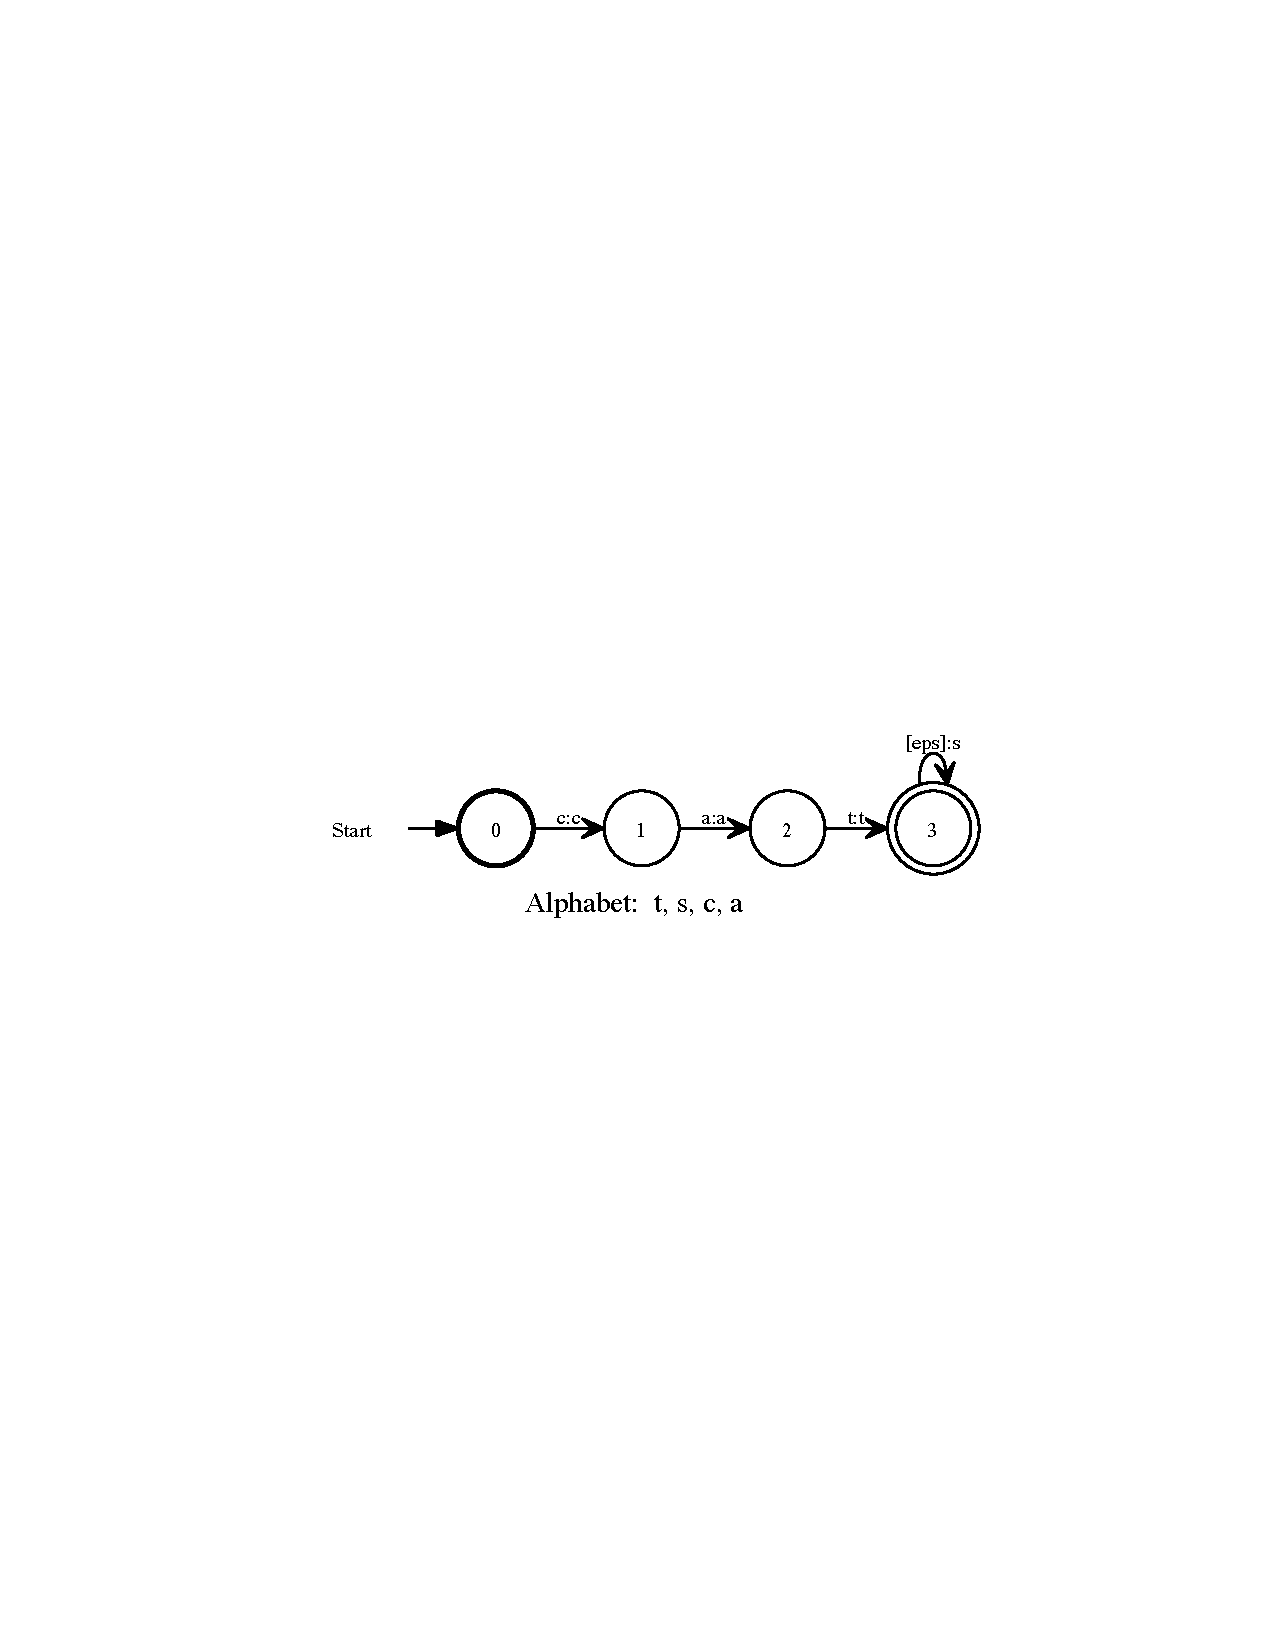
\includegraphics{images/inputepscycle.pdf}
\end{center}

\noindent
If this \fsm{} is applied in a downward direction to \emph{cat}, i.e.\@ if the input string
\emph{cat} is matched against the upper/input side, the input side epsilon cycle on node 3
allows an infinite number of matches, with an infinite number of outputs:

\begin{alltt}
cat
cats
catss
catsss
catssss
\ldots{}
\end{alltt}

To test your \fsm{} for cycles, use the
pre-defined boolean predicate \verb!#^isIBounded()! (for ``is input bounded''), which is aliased as
\verb!#^isUBounded()! (for ``is upper bounded'').
For example, in the Kleene \gui{}, if your \fsm{} is named \verb!$Fst!, just do the
following:

\begin{Verbatim}
#bool = #^isIBounded($Fst) ;
\end{Verbatim}

\noindent
or equivalently

\begin{Verbatim}
#bool = #^isUBounded($Fst) ;
\end{Verbatim}

\noindent
and the system will respond indicating 1 (= true = input/upper bounded)
or 0 (= false = the \fsm{} has input/upper epsilon cycles).   
You could be a little fancier and write

\begin{Verbatim}
if (#^isIBounded($Fst))
    pr "OK.  It's input bounded." ;
else
    pr "DANGER: There are input epsilon cycles." ;
}
\end{Verbatim}

\noindent
Again, you
probably do \emph{not} want input/upper cycles in your \fsm{}.  If you proceed with an \fsm{}
that has input epsilon cycles, the generated Java code should look
for and block epsilon loops, but this feature is still experimental.

\subsubsection{Step Four: Output the \fsm{} as a State-Oriented \xml{} file}

Beware: there are currently two quite separate ways to output a Kleene \fsm{} as \xml{}:

\begin{enumerate}
\item
An arc-oriented format using the command \texttt{writeXml}; this
	\xml{} format can be read back into Kleene using the \texttt{readXml} command, and
\item
A state-oriented \xml{} format using the command \texttt{writeXmlStateoriented}
\end{enumerate}

\noindent
For use with fst2java, you want the second (state-oriented) output.

Output your \fsm{} to file in the special state-oriented \xml{} format
using the command \texttt{writeXmlStateOriented}.  If your \fsm{} is named
something other than \verb!$Fst!, substitute ``Fst'' with your own \fsm{}'s name in
the following command:

\begin{Verbatim}
writeXmlStateOriented $Fst, "Fst.xml", "UTF-8" ;
\end{Verbatim}

\noindent
This command creates a file named \texttt{Fst.xml} in the current directory.
This file contains a state-oriented representation of your \fsm{} in an
\xml{} format.  Don't worry too much about this right now---it just means that \xml{} elements
representing the arcs exiting a state are grouped inside another \xml{} element
representing that state.) The challenge is now to take this \texttt{Fst.xml}
file (or whatever you have called it) and generate from it executable
Java code that simulates the application of the original \fsm{}.

\subsubsection{Step Five:  Generating the Java Package using fst2java}

Now \texttt{cd} to the fst2java directory (downloadable from
\url{www.kleene-lang.org}), which contains four \xslt{} scripts that
convert the \fsm{} from one form of \xml{} to another form of \xml{}, plus one
final \xslt{} script, named \texttt{generate\_java.xsl}, that takes the final \xml{}
file and generates from it the Java code as a Java package.\footnote{A Java package is a set of related Java files residing in
one directory.}  The
application of these five \xslt{} scripts is all controlled by the Makefile
in the fst2java directory, so we're very close to the end.

Java packages need to have a name, so you now have to
choose the name.  I assume
here that you want to call it ``Fst,'' but choose any name that you like.

If you want to use the name ``Fst,'' then do exactly one of three things:

\begin{enumerate}
\item
Move your just-generated \texttt{Fst.xml} file to the fst2java directory, or
\item
Copy your \texttt{Fst.xml} file to the fstjava directory, or
\item
Create a soft link named \texttt{Fst.xml}, in the fst2java directory, to \texttt{Fst.xml}
\end{enumerate}

\noindent
It doesn't really matter which one you choose.  If in doubt, just create
the soft link.  Here's how to create a soft link (fixing the paths to reflect your environment as
appropriate):

\begin{Verbatim}
$ cd /path/to/fst2java
$ ln -s /path/to/Fst.xml
\end{Verbatim}

If you want the Java class to be named something else, such as
``MyMorphology,'' then do exactly one of these three things:

\begin{enumerate}
\item
Move your \texttt{Fst.xml} (or whatever you called it) file to the
	fst2java directory and rename it \texttt{MyMorphology.xml}, or
\item
Create a copy of \texttt{Fst.xml} in the fst2java directory and call that
	copy \texttt{MyMorphology.xml}, or
\item
Create a soft link, named \texttt{MyMorphology.xml}, in the fst2java directory, 
linking it to \texttt{Fst.xml}
\end{enumerate}

\noindent
If in doubt, just create a soft link.  Here's how to create a soft link
named \texttt{MyMorphology.xml}

\begin{Verbatim}
$ cd /path/to/fst2java
$ ln -s /path/to/Fst.xml MyMorphology.xml
\end{Verbatim}

\subsubsection{Step 6: Validate the \xml{} File}

From this point on, you will be using the Makefile in the fst2java directory, and that Makefile depends on
having Java, the \init{jdk} (Java Development Kit),\footnote{If you are running Kleene, you have the \init{jre} Java Runtime
Environment, but you may not have the \init{jdk} (Java Development Kit), which includes the
\texttt{javac} compiler.} and two Java \acro{jar} files, installed in your environment.

To see if you have the \init{jdk} installed, enter

\begin{Verbatim}
$ which javac
\end{Verbatim}

\noindent
Hopefully, the system will return a path showing where \texttt{javac} is installed.  If the command fails, returning a message like
``Command not found,'' then you will first need to install the \init{jdk}.  If
this means nothing to you, consult your system administrator or a Java-savvy friend.

Now, in the fst2java directory, edit the Makefile, using a plain-text editor like emacs, vim, vi, gedit, etc.\@ and note the two definitions at the top:

\begin{Verbatim}
SAXONJAR=/Users/beesley/java/saxon/saxon.jar
# This is a comment.
# Edit the SAXONJAR path above to point to your copy of 
#   saxon.jar, which may be named saxon9he.jar
# If you don't have saxon.jar, see 
# 	http://saxon.sourceforge.net/
# and download the Saxon-HE (home edition), 
#  which contains the jar file.

JINGJAR=/Users/beesley/java/jing/bin/jing.jar
# Edit the JINGJAR path above to point to your copy 
#	of jing.jar
# If you don't have jing.jar, see 
# http://code.google.com/p/jing-trang/downloads/list
# and download jing-20091111.zip or a newer version.
\end{Verbatim}

\noindent
As of this writing, the current version of Saxon is SaxonHE9-5-0-1J and the actual \acro{jar} file in the download is
named \texttt{saxon9he.jar}.  Save this \acro{jar} file in a convenient location and edit the Makefile so that the definition of
\texttt{SAXONJAR} points to the \acro{jar} file on your system.  For example, if your name is Victoria and you store the \acro{jar} file in
\texttt{/home/victoria/javajars/}, edit the line to

\begin{Verbatim}
SAXONJAR=/home/victoria/javajars/saxon9he.jar
\end{Verbatim}

Similarly, you need \texttt{jing.jar}.  If you don't have it already, surf to \url{/http://code.google.com/p/jing-trang/downloads/list} and
download \texttt{jing-20091111.zip} (or a newer version, if any).  If necessary, unzip the file (sometimes this is done by
your browser during the download).  Inside the resulting \texttt{jing-20091111-1} directory, inside the \texttt{bin}
subdirectory, is the \texttt{jing.jar} file.  Save this file in a
convenient location and edit the definition of \texttt{JINGJAR} in
the Makefile to show the path to it on your system.  Save the Makefile.

As a first test, let's try to validate your \texttt{Fst.xml} file, or whatever it's called.\footnote{The validation is
performed against a Relax NG schema named fst.rnc, which is supplied in the fst2java
directory.}  Validation (using the Makefile and the supplied Relax NG script) requires Java and the
\texttt{jing.jar} file.  Enter the following command:

\begin{Verbatim}
$ make name=Fst validate
\end{Verbatim}

\noindent
If your file (or soft link) is name something else, such as \texttt{BobsFirstTry.xml}, then change the command to

\begin{Verbatim}
$ make name=BobsFirstTry validate
\end{Verbatim}

\noindent
If there is no response, simply a return to the command-line prompt, then all is well.  If the command itself fails to run,
then there is some problem with your Java or jing.jar installation.  Review the instructions above and/or consult an expert.
If the validation starts but reports errors in the \xml{} file, then please contact me (krbeesley@gmail.com) with a detailed
error report.  You won't be able to progress with code generation until the problem is solved.

If the validation is successful, then enter

\begin{Verbatim}
$ make name=Fst
\end{Verbatim}

\noindent
changing the name as appropriate.  If all goes well, it will generate a Java package in a new directory
named \texttt{FstPackage}.

If your \xml{} file (or link) is named something else, like \texttt{BobsFirstTry.xml}, then launch

\begin{Verbatim}
$ make name=BobsFirstTry
\end{Verbatim}

\noindent
and it will generate a Java package in a directory named BobsFirstTryPackage.

\subsection{\fsm{} to Java Examples}

\subsubsection{A Simple Alternation Rule}

Congratulations on making it this far.  It's time for some practical examples.  Let's start with a simple alternation rule
that maps \emph{s} to \emph{z} when it occurs between two vowels.  In the Kleene \gui{}, define the following rule:

\begin{Verbatim}
$Vowel = [aeiou] ;
$StoZrule = s -> z / $Vowel _ $Vowel ;
\end{Verbatim}

\noindent
or just

\begin{Verbatim}
$StoZrule = s -> z / [aeiou] _ [aeiou] ;
\end{Verbatim}

\noindent
As previously noted, alternation rules compile into transducers, and a right-arrow rule has an inherent downward-oriented (or
generation) bias
built into it.   The way the rule is written, we naturally think of applying it in a downward direction to an input string
like \emph{casa} and getting back \emph{caza} as the output.   That is, the input is matched against the upper side (the Openfst
``input'' side), and the output is read off of the lower side of the matched paths(s).  Now let's test the rule, still in the Kleene \gui{}:


\begin{Verbatim}
test $StoZrule ;
\end{Verbatim}

\noindent
A test window will pop up, and we enter \emph{casa} in the upper-side text-entry field.  When we press Enter, the answer

\begin{Verbatim}
caza: 0.0
\end{Verbatim}

\noindent
appears in the history window.  Now enter
\emph{sasusis} in the upper-side entry field and the output, as expected, is

\begin{Verbatim}
sazuzis: 0.0
\end{Verbatim} 

Let's assume that we want to generate Java code that will have this same
downward-oriented behavior, a ``generation'' behavior, matching input
against the upper side, with the output read off of the lower side.  
This reflects the OpenFst notion of input side,
and so everything is already in the proper orientation for code generation.  We do \emph{not} want
to invert this \fsm{} before Java-code generation.

Before we proceed to generate Java code, let's take a look at the \fsm{}.

\begin{Verbatim}
draw $StoZule ;
\end{Verbatim}


\begin{center}
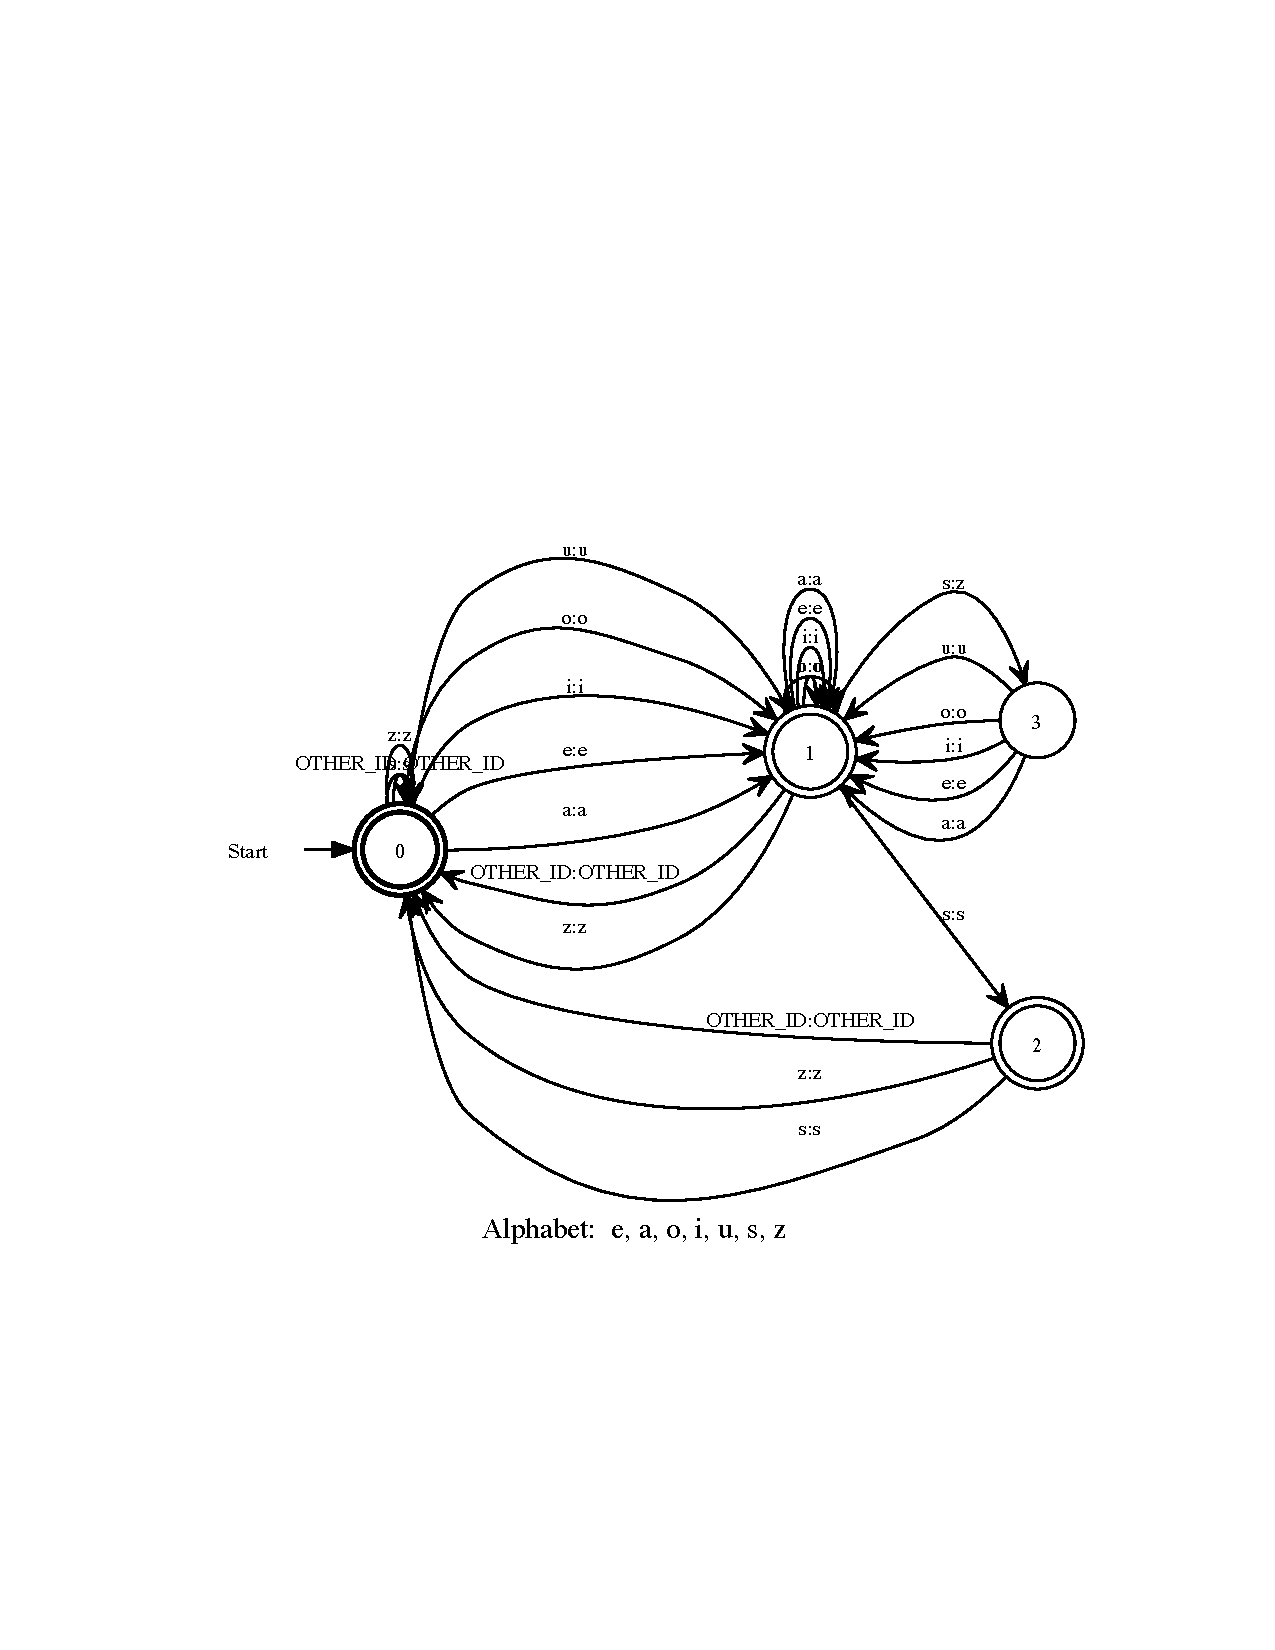
\includegraphics[scale=0.9]{images/StoZrule.pdf}
\end{center}


\noindent
Note that the \fsm{} has three states, numbered 0, 1 and 2, and we'll see this structure reflected in the generated Java code.
We also test the \fsm{} for input-side boundedness

\begin{Verbatim}
if (#^isIBounded($StoZrule))
    pr "All is OK" ;
else
    pr "Problem: input epsilon cycle(s)" ;
\end{Verbatim}

\noindent
The system responds with ``All is OK'' and we can proceed.

Now we output the the rule \fsm{} to file in the state-oriented \xml{} format:

\begin{Verbatim}
writeXmlStateOriented $StoZrule, "StoZrule.xml", "UTF-8" ;
\end{Verbatim}

\noindent
This will create file \texttt{StoZrule.xml}.  Now \texttt{cd} to the
fst2xml directory, create a soft link to the \texttt{StoZrule.xml}
file just created, and validate the file just to be sure that it's
kosher.

\begin{Verbatim}
$ cd /path/to/fst2xml
$ ln -s /path/to/StoZrule.xml
$ make name=StoZrule validate
\end{Verbatim}

If the validation is successful, i.e.\@ if it returns silently, 
we can, finally, generate the Java code:

\begin{Verbatim}
$ make name=StoZrule
\end{Verbatim}

\noindent
You should now see a newly created directory named \texttt{StoZrulePackage}
that contains the central Java source-code
file \texttt{StoZRule.java} plus an \texttt{s}\emph{N}\texttt{.java}
file for each state in the original \fsm{}, where N is 0 \ldots{} n.
When we drew the \fsm{} earlier, we saw that there were three states,
and in \texttt{StoZrulePackage} we see \texttt{s0.java},
\texttt{s1.java} and \texttt{s2.java} representing those three states.

\begin{Verbatim}
$ cd StoZrulePackage
$ ls
StoZrule.java s0.java s1.java s2.java
\end{Verbatim}

The new Java class \texttt{StoZrule} can be imported and used inside any Java
program.  Type the following minimal example into a file named
\texttt{Test.java} in the same directory where \texttt{StoZrulePackage} resides.

\begin{Verbatim}
// Test.java
// For testing fst2java for Kleene FSMs

import java.util.Scanner ;
// import the new package/class
import StoZrulePackage.StoZrule ; 

public class Test {
  public static void main(String[] args) {
    String result ;

    // create an instance of the StoZrule class
    StoZrule rule = new StoZrule() ;

    // create an instance of Scanner to read
    //    input from the terminal
    Scanner scanner = new Scanner(System.in) ;
    while (true) {
      // output a prompt
      System.out.print("Enter input string: ") ;
      // read the input string entered by the user
      String input = scanner.nextLine().trim() ;

      // if the input string is 'quit' or 'exit',
      //    then exit the loop and terminate
      if (input.equals("quit") || input.equals("exit"))
          break ;

      // call the xapply(String) method of StoZrule,
      //    one of several available methods
      result = rule.xapply(input) ;

      System.out.println(result) ;
    }
  }
}
\end{Verbatim}

\noindent
This particular example creates an instance of \texttt{StoZrule}, named \texttt{rule}, gets an input
string entered by the user (you), and applies \texttt{StoZrule}'s xapply() method to that input string.  The method call returns an output string in an \xml{}
format and prints it to the terminal.   

\begin{Verbatim}
<results>
  <result><str>caza</str><w>0.0</w></result>
</results>
\end{Verbatim}

In addition to \texttt{xapply(String str)} there are several other
application methods available; these methods and the \xml{} format
will be documented below.

To compile the Java file, use the \texttt{javac} command:\footnote{If your system does not have
\texttt{javac}, you need to install the \init{jdk}, the Java Development Kit.  See your system
administrator or a Java-savvy friend.}

\begin{Verbatim}
$ javac Test.java
\end{Verbatim}

\noindent
This creates a file named \texttt{Test.class}, which you can run with the \texttt{java} command.

\begin{Verbatim}
$ java Test
\end{Verbatim}

\noindent
The system will then display the prompt, wait for you to type a string and press the Enter key,
print the result, and then re-display the prompt for the next input.  Try entering \emph{casa}.

\begin{alltt}
Enter input string: \emph{casa}
caza
Enter input string:
\end{alltt}

\noindent
Then try entering other words such as \emph{elephant}, \emph{sopa}, \emph{sasesisosus}, etc.\@ to
make sure that the output is correct, mapping all (and only) \emph{s}s that appear between two
vowels into \emph{z}.  Note that when a word does not contain an \emph{s} at all (such as
\emph{elephant}), and when a word contains an \emph{s}, but not between two vowels (as in
\emph{sopa}), the input string is mapped to the output without change---the rule simply does not
apply to such strings.

Enter \emph{exit} or \emph{quit} to break the loop and terminate the program.

\subsubsection{An Esperanto Verb Example}

As a second example, we will build a small morphological analyzer \fst{} that models a fragment of
Esperanto verbs.  In particular, we'll model verbs that start with an optional prefix \emph{mal},
meaning opposite, or \emph{ne}, meaning negative; followed by a required verb root; followed by
an optional aspect marker suffix \emph{ad}, indicating repetitive/habitual/imperfect; followed
by a required verb suffix indicating tense/mood.  Type the following into a Kleene script file, named
something like \texttt{EspVerb.kl}.

\begin{Verbatim}
// EspVerb.kl
$vpref = '[Op]':(mal) | '[Neg]':(ne) ; // opposite, negative
$vroot = pens | don | ir | dir | est ;
//     think    give  go   say   be
$vrep = '[Rep]':(ad) ;      // repetitive aspect/imperfect
$vend = '[Pres]':(as) |     // present tense
        '[Past]':(is) |     // past tense
        '[Fut]':(os) |      // future tense
        '[Cond]':(us) |     // conditional
        '[Subj]':u |        // subjunctive
        '[Inf]':i ;         // infinitive

$EspVerb = $vpref? $vroot '[Verb]':"" $vrep? $vend ;
\end{Verbatim}

\noindent
and then, inside the Kleene \gui{}, invoke

\begin{Verbatim}
source "EspVerb.kl" ;
test $EspVerb ;
\end{Verbatim}

This will bring up the now-familiar testing window, and let's assume that that want to test this
\fsm{} in analysis mode, applying it in an upward direction to surface orthographical
strings like \emph{estos} and \emph{donadis}, getting
back analysis strings like \emph{est[Verb][Fut]} and \emph{don[Verb][Rep][Past]}, respectively.  
To do this we enter strings like
\emph{donadis} in the \emph{lower} input field of the testing window so that they are matched against the lower side of the
\fsm{}, and the results are read off of the upper side of the matched path(s).
Test examples like \emph{estas}, \emph{estis}, \emph{malpensos}, \emph{neestos}, \emph{irus}, \emph{diri}  and \emph{donu}.

To generate Java code that performs this same upward-oriented analysis, recall that the Java
code always matches input strings against what was the \emph{upper} side of the \fsm{}, what
OpenFst called the ``input'' side.  This \fsm{} is effectively upside-down for our intended
purpose; so before we generate the Java code, we need to invert this particular \fsm{}, and we
could call the result something like \verb!$EspVerbInv! or \verb!$EspVerbAnalyze!.

\begin{Verbatim}
$EspVerbAnalyze = $^invert($EspVerb) ;
\end{Verbatim}

\noindent
And then we can test the result

\begin{Verbatim}
test $EspVerbAnalyze ;
\end{Verbatim}

\noindent
noting that now we enter strings like \emph{malpensos} in the \emph{upper} input field of the
test window.  This is the orientation we need before we generate the Java code.

Now we generate the state-oriented \init{xml} file in the usual way:

\begin{Verbatim}
writeXmlStateOriented $EspVerbAnalyze, "EspVerbAnalyze.xml", "UTF-8" ;
\end{Verbatim}

\noindent
We then exit Kleene, \texttt{cd} to the fst2java directory and in a command-line terminal do the
following:

\begin{Verbatim}
$ ln -s /path/to/EspVerbAnalyze.xml
$ make name=EspVerbAnalyze validate
$ make name=EspVerbAnalyze
\end{Verbatim}

\noindent
The result will be a directory named \texttt{EspVerbAnalyzePackage} containing
\texttt{EspVerbAnalyze.java} and a Java file for each state in the original \fsm{}.  
We can test this in
Java using the following code, which now uses \texttt{EspVerbAnalyze} where we previously had
\texttt{StoZrule}.

\begin{Verbatim}
import java.util.Scanner ;
import EspVerbAnalyzePackage.EspVerbAnalyze ;

public class Test {
  public static void main(String[] args) {
    String result ;

    EspVerbAnalyze esp = new EspVerbAnalyze() ;

    Scanner scanner = new Scanner(System.in) ;
    while (true) {
      System.out.print("Enter input string: ") ;
      String input = scanner.nextLine().trim() ;
      if (input.equals("quit") || input.equals("exit"))
        break ;

      // call the xapply(String) method of EspVerbAnalyze
      result = esp.xapply(input) ;

      System.out.println(result) ;
    }
  }
}
\end{Verbatim}

Compile and run the program as shown for the \texttt{StoZrule} example above, and you should be
able to enter strings like \emph{donadis} and get back strings like \emph{don[Verb][Rep][Past]}.
[KRB: test and show output in XML]



\subsubsection{Multiple Output Example}

In some languages, certainly including English, many orthographical words are ambiguous,
requiring a morphological analyzer to return multiple results.  Consider the following example
that models a small fragment of English morphotactics with some ambiguities:

\begin{Verbatim}
$vroot = think | look | file ;
$nroot = desk | look | file ;
$nouns = $nroot '[Noun]':"" ( '[Sg]':"" | '[Pl]':s ) ;
$verbs = $vroot '[Verb]':"" 
                ( '[Bare]':"" | '[3PS]':s | '[PresP]':(ing) ) ;

$Eng = $nouns | $verbs ;
\end{Verbatim}

\noindent
This grammar captures the fact that words like \emph{look} and \emph{files} are ambiguous,
being either a noun or a verb.  If we compile this little grammar in Kleene, creating
\verb!$Eng!, and then test it manually:

\begin{Verbatim}
test $Eng ;
\end{Verbatim}

\noindent
we can enter \emph{files} in the \emph{lower} input field and get back two solutions:


\begin{Verbatim}
file[Noun][Pl]
file[Verb][3PS]
\end{Verbatim}

Note that this \fsm{}, as we have built it, has analysis strings on the upper side, and
orthographical strings on the lower side.  Assuming that we want to generate Java code that
performs analysis, mapping from orthographical strings to analysis strings, we will need to
invert this \fsm{} before generating the state-oriented \xml{} output file.


\begin{Verbatim}
$EngAnalysis = $^invert($Eng) ;
writeXmlStateOriented $EngAnalysis, "EngAnalysis.xml", "UTF-8" ;
\end{Verbatim}

If you follow the steps of the previous examples to generate the Java code and modify the Java test script to
run it, you should be able to enter \emph{files} and get back


\begin{Verbatim}
<results>
  <result><str>file[Noun][Pl]</str><w>0.0</w></result>
  <result><str>file[Verb][3PS]</str><w>0.0</w></result>
</results>
\end{Verbatim}

\noindent
showing that the orthographical word \emph{files} can be analyzed either as a plural noun or a
third-person-singular verb.

The generated Java code contains other methods that return the results not as \xml{} but as an
ArrayList of String, as in the following example:

\begin{Verbatim}
import java.util.Scanner ;
import EspVerbAnalyzePackage.EspVerbAnalyze ;

public class Test {
  public static void main(String[] args) {
    ArrayList<String> result ;  // note the ArrayList here

    EspVerbAnalyze esp = new EspVerbAnalyze() ;

    Scanner scanner = new Scanner(System.in) ;
    while (true) {
      System.out.print("Enter input string: ") ;
      String input = scanner.nextLine().trim() ;
      if (input.equals("quit") || input.equals("exit")) break ;

      // call the apply(String) method of EspVerbAnalyze
      // Note that examples above used the xapply(String str)
      //    method.
      result = esp.apply(input) ;

      // iterate through the results in the ArrayList, if any, 
      //    and print them out
      if (result.isEmpty())
        System.out.println("***No Results***") ;
      else 
        for (String item: results)
          System.out.println(item) ;
    }
  }
}
\end{Verbatim}

The methods that return ArrayList, as well as those that return an \xml{} String, are all
documented below.

\subsection{Generated Java Code \init{api}}

\subsubsection{Methods that Return an ArrayList of String}

The generated Java class file contains the following public methods, all of which match the
input string on the ``input'' side of the original \fsm{}, but they differ in the way that the
results are returned.

\begin{Verbatim}
public ArrayList<String> apply(String str)
\end{Verbatim}

\noindent
This method tokenizes the input string (looking for multi-character symbols),
applies the \fsm{} to the String argument,\footnote{More precisely, the string is converted to
a list of integer code point values, and the \fsm{} is effectively applied to that list of code
point values.}  and returns the result(s) as 
an ArrayList of String.  An output label \acro{other\_nonid} in the original \fsm{} is
represented as \emph{?} (the normal question mark) and the
string output is separated from the weight by \emph{::} (two colons).

\begin{Verbatim}
public ArrayList<String> apply(String str, 
                               Boolean tokenizeInputString)
\end{Verbatim}

\noindent
As for \texttt{apply(String str)} except that the second argument controls whether tokenization
(to look for multi-character symbols) is performed.  If the input strings are surface,
orthographical strings, then they typically contain no multi-character symbols, and the
tokenization step can be skipped, improving performance.

\begin{Verbatim}
public ArrayList<String> apply(String str, 
                               String other_nonid)
\end{Verbatim}

\noindent
As for \texttt{apply(String str)} except that the second argument indicates how an output label
\acro{other\_nonid} should be displayed in output strings.  (The default, when calling
\texttt{apply(String str)} is \emph{?}.

\begin{Verbatim}
public ArrayList<String> apply(String str, 
                               String other_nonid, 
                               Boolean tokenizeInputString)
\end{Verbatim}

\noindent
As for \texttt{apply(String str)} except that the second argument indicates how
\acro{other\_nonid} should be displayed, and the third argument controls whether tokenization (to
look for multi-character symbols) is performed.

\begin{Verbatim}
public ArrayList<String> apply(String str, 
        String other_nonid,
        String mcs_start, String mcs_end, 
        String str_start, String str_end,
        String weight_start, String weight_end,
        Boolean tokenizeInputString)
\end{Verbatim}

\noindent
As in the examples above, plus additional arguments to specify custom markup:  \texttt{mcs\_start} and
\texttt{mcs\_end} indicate strings to surround multi-character symbols; \texttt{str\_start} and
\texttt{str\_end} indicate strings to surround string outputs, and \texttt{weight\_start} and
\texttt{weight\_end} indicate strings to surround the weights.

\subsubsection{Methods that Return an \xml{} String}

The following methods return the results as a single \xml{} String.

\begin{Verbatim}
public String xapply(String str)
\end{Verbatim}

\noindent
This method returns a String in an \xml{} format.  When
the output has exactly one string, the following structure is returned (whitespace added here for human
readability):

\begin{alltt}
<results>
  <result><str>\emph{string}</str><w>\emph{weight}</w></result>
</results>
\end{alltt}

\noindent
If the output contains two results, then the structure is (again with added whitespace for
readability)

\begin{alltt}
<results>
  <result><str>\emph{string}</str><w>\emph{weight}</w></result>
  <result><str>\emph{string}</str><w>\emph{weight}</w></result>
</results>
\end{alltt}

\noindent
and similarly for three or more results.  A multi-character symbol is returned inside
\texttt{<mcs>}\ldots\texttt{</mcs>} tags, and any \acro{other\_nonid} output symbol is represented as
\texttt{<other/>}.

\begin{Verbatim}
public String xapply(String str,
                     Boolean tokenizeInputString)
\end{Verbatim}

\noindent
As for \texttt{xapply(String str)} except that \texttt{tokenizeInputString} controls whether
the input string is tokenized (to look for multi-character symbols).  If the input strings are
orthographical strings, which typically do not contain multicharacter symbols, then
tokenization is not required and
\texttt{tokenizeInputString} can be set to \emph{false} for better performance.

\begin{Verbatim}
public String xapply(String str, 
                     String other, 
                     String mcs_tag, 
                     String str_tag, 
                     String weight_tag, 
                     String result_tag, 
                     String results_tag, 
                     Boolean tokenizeInputString)
\end{Verbatim}

\noindent
As above except that additional argument allow the user to control the spelling of the \xml{}
tags.  For example, if the \texttt{other} value is ``unknown'', then any \acro{other\_nonid} output
symbol will be represented in the \xml{} as \texttt{<unknown/>}.  If \texttt{mcs\_tag} is ``mult'',
then any multi-character symbols in the output will be surrounded with
\texttt{<mult>}\ldots\texttt{</mult>}.  Similarly, \texttt{str\_tag} specifies the spelling of
the tags surrounding string outputs, \texttt{weight\_tag} specifies the spelling of the tags
surrounding weights, \texttt{result\_tag} specifies the spelling of the tags surrounding each
result, and \texttt{results\_tag} specifies the spelling of the top-level \xml{} tags surrounding
all the results.

\section{Runtime Code}

\subsection{Status of Runtime Code}

There is currently no traditional runtime code available for running Kleene \fsm{}s.  Perhaps
some interested readers would be interested in writing such code.  This section give a
high-level overview of what runtime code would do.

See the section
above entitled ``The fst2java Experiment'' for a way to convert a Kleene \fsm{} into a
Java class that can be imported and used by any Java program or any other language (Scala,
Groovy, Clojure) that is based on the Java Virtual Machine (\init{jvm}).\footnote{Programs in Java, Scala, Groovy and Clojure are compiled into
\emph{byte-code} that is then interpreted by the \init{jvm} (Java Virtual Machine) at runtime.  \init{jvm} programs run on all popular platforms and operating systems.}

\subsection{Basic Functionality of Runtime Code}

If we have built an \fsm{} in Kleene and saved it to file as \init{xml} (or some similar markup
language), runtime code is
code, external to Kleene itself, that would perform the following tasks:

\begin{enumerate}
\item
Read the \init{xml} file representing a Kleene \fsm{} and build a
representation of that \fsm{} in memory
\item
Accept input in the form of a string
\item
Convert the input string into a list of Unicode code point values, taking account of
any multi-character symbols in the alphabet of the \fsm{}
\item
Apply the \fsm{} to the list of code point values (representing the input string)
\item
Collect the output string or strings, and
\item
Return them in an appropriate form to the caller
\end{enumerate}

\noindent
The application capabilities might include \emph{downward application} and/or \emph{upward
application}.  Downward application involves matching the list
of code point values (representing the input string) against paths of labels on the upper (OpenFst ``input'') side of the
\fsm{}, and returning the lists of labels on the lower (OpenFst ``output'') side of the
matched paths.  Conversely, upward application involves matching the list of code point
values against paths of labels on the lower (OpenFst ``output'') side of the \fsm{}, and
returning the lists of labels on the upper (OpenFst ``input'') side of the matched paths.

The runtime code would typically be implemented as a library, for
example a \CPP{} library that
could be loaded
by a \CPP{} program.  The library would have an \init{api} listing the callable functions of the library
that implement the tasks just listed.  Any larger program that imported the
runtime-code library would be able to integrate \fsm{} processing.

\subsection{Kinds of Runtime Code}

\subsubsection{Complete Match}

\fsm{}s can be used in several modes, and different modes may require different kinds of runtime
code.  The most straightforward way to use \fsm{}s involves taking an input string (or a
list of code point values computed from that string) and looking for \emph{complete
matches} of those code point values against complete paths of arc labels in the \fsm{}.  A
complete or full match starts at the \fsm{}'s start state and ends at one of the \fsm{}'s final states, with none of
the input string's symbols (code point values) remaining unmatched.  Full matching
behavior is typical of applications including

\begin{itemize}
\item
Tokenization
\item
Phonological modeling
\item
Morphological analysis and generation
\end{itemize}

\noindent
In morphological analysis, for example, the input is typically a string representing an
orthographical word, and the entire string should completely match a path in the \fsm{}.

\subsubsection{Partial Match}

Another desirable modality in many applications is to view the \fsm{} as a union of patterns to be
matched anywhere inside the input string, which might be a long file.  This could be called
\emph{partial matching} because any given pattern need match only part of the input string.  Many
patterns/paths in the \fsm{} might match somewhere inside the input string, and any single pattern/path
in the \fsm{} might match multiple times inside the input string.  Parts of the input string---which,
again, might be long file---may not be matched by any pattern.  Partial matching behavior is typical of
applications such as

\begin{itemize}
\item
Entity extraction, e.g.\@ finding names of people, companies, countries, etc.\@ in an
input text
\item
Sentiment analysis
\item
Shallow/robust parsing
\end{itemize}

One possible strategy for partial-matching is to implement runtime code that
begins by setting a \emph{match pointer} at the beginning of the input string and trying
to find a pattern from the \fsm{} that matches at least part of the input string, starting at the
match pointer.  If a single pattern matches, then the start and end of the match is
stored as a result/success, the match pointer is advanced to the end of the matched input
segment, and the
matching procedure is
restarted from that new point.  If no patterns match, then the match pointer is
advanced to the next symbol or word, as appropriate for the application.  If multiple
patterns match starting at the same match point in the input, then the runtime code might be
written to record all matches, or to prefer the longest match.
Many variations in matching behavior are possible, depending on the demands of the larger
application.  

Eventually, it would be useful to have runtime code to implement complete-matching and
partial-matching strategies for Kleene \fsm{}s, perhaps in several semantic variations and in
several computer languages, to allow \fsm{}-based functionality to be integrated into arbitrary
software applications.  The difficulty of writing correct and robust runtime code should not be
underestimated, and runtime code must be highly tuned to achieve maximum performance.

